\documentclass[11pt,a4paper]{article}
\usepackage[margin=2.4cm]{geometry}
\usepackage{amsmath,amssymb}
\usepackage{graphicx}
\usepackage{booktabs}
\usepackage{listings}
\usepackage{xcolor}
\usepackage[colorlinks=true,linkcolor=blue!50!black,citecolor=blue!50!black,urlcolor=blue!50!black]{hyperref}
\usepackage{natbib}
\lstset{basicstyle=\ttfamily\scriptsize,columns=fullflexible,breaklines=true,
        frame=single,rulecolor=\color{gray!50},keywordstyle=\color{blue!60!black},
        commentstyle=\color{green!40!black},language=Python,showstringspaces=false}
\newcommand{\dd}{\mathrm{d}}
\newcommand{\Rb}{R_b}
\newcommand{\rsp}{r_{\rm sp}}
\newcommand{\rta}{r_{\rm ta}}

\title{Splashback and the accretion front\\[4pt]
\large A companion note to \emph{From a primordial fluctuation to an idealised rotation curve}}
\author{B. R. Parodi}
\date{23 October 2026}

\begin{document}
\maketitle

\begin{abstract}
In simulated dark-matter haloes the orbits of freshly accreted matter
end at the splashback radius, where the density profile drops steeply
and which separates matter that already orbits the halo from matter
still falling in. Our model has a similar two-part structure: a settled
galaxy inside the accretion front $\Rb$ and shells on their first infall
outside it. We explain splashback for a graduate reader, place our seed
in its language, and measure the splashback radius of our own seed with
a one-dimensional collisionless shell code. The front and the splashback
radius are related but not identical: the profile of the collisionless
run drops most steeply at $1.17\,\Rb$, and its orbiting matter extends
to $1.6\,\Rb$, in agreement with the calibration of simulated haloes. Our
front is thus the inner edge of the splashback zone, close to the
classical virial radius. About 15\% of the orbiting matter lies outside
the front, which confirms the estimate of the unrelaxed layer in the
energy budget of the main paper.
\end{abstract}

\section{What splashback is}

Take a shell of dark matter that turns around and falls into a halo.
Without collisions it does not stop: it falls through the centre, comes
out on the other side, and reaches a first apocentre before falling back
again. Because all shells that turn around at about the same time follow
nearly the same orbit, their first apocentres pile up at one radius,
where the density has a caustic. This radius is the splashback radius
$\rsp$ \citep{Diemer2014,Adhikari2014,More2015}. Inside it, matter moves
on many streams, in and out; outside it, there is only the single stream
of matter on its first infall. In a smooth spherical model the caustic
is a density spike; in real haloes, with a spread of orbits and
non-spherical accretion, it becomes a sharp steepening of the density
profile, with logarithmic slopes of $-3$ to $-4$ or steeper, located at
\begin{equation}
  \rsp\simeq(0.8\text{--}1.5)\,R_{\rm 200m},
\end{equation}
where $R_{\rm 200m}$ encloses 200 times the mean matter density. The
ratio depends mainly on the mass accretion rate
$\Gamma=\dd\ln M/\dd\ln a$: fast accretion deepens the potential while a
shell is out at apocentre and pulls the apocentre in, so rapidly
accreting haloes have $\rsp\approx0.8$--$1\,R_{\rm 200m}$ and slowly
accreting ones $\rsp\approx1.5\,R_{\rm 200m}$ \citep{More2015}.

\citet{Diemer2022} turned this into a description of the whole profile.
He counts the pericentric passages of every particle and splits the
density into an \emph{orbiting} term (at least one pericentre) and an
\emph{infalling} term (none). The orbiting term is truncated sharply near
$\rsp$ and depends mostly on the accretion rate; the infalling term
continues outwards and depends mostly on the environment.

\section{Our seed in the language of splashback}

\paragraph{The same two parts.} In the main paper the density during
growth is one function, $\rho=P(R/vt)/Gt^2$ (its Sect.~5.1): the P18
profile inside the accretion front $\Rb=\xi_bvt$, $\xi_b=1/(1+3\pi/2)$,
and the density of the shells on their first infall outside it, with a
jump by a factor 6.7 at the front. This is the orbiting-plus-infalling
decomposition of \citet{Diemer2022}, with two differences: our inner part
is \emph{settled} rather than orbiting, and our boundary is a
discontinuity rather than a steep but continuous drop.

\paragraph{Accretion rate.} Every shell of our seed has the same energy,
so it turns around at $t_{\rm ta}=\pi GM/v^3\propto M$: the halted mass
grows as $M\propto t$. In an Einstein--de Sitter background, $a\propto
t^{2/3}$, this is $\Gamma=\dd\ln M/\dd\ln a=3/2$, a moderate accretion
rate typical of dwarf haloes. In the classification of
\citet{Fillmore1984}, whose initial overdensities fall as
$\delta\propto M^{-\epsilon}$, our seed has $\epsilon=2/3$, the case
that gives an isothermal profile, $\rho\propto r^{-2}$, and hence a flat
rotation curve. \citet{Bertschinger1985} treated $\epsilon=1$, a slower
accretion ($\Gamma=1$) with a slightly steeper profile; his
collisionless solution has its outermost caustic at about a third of the
current turnaround radius.

\paragraph{Where does our front sit?} The halted shell of mass $M$ stops
at half its own turnaround radius, at $1.82\,t_{\rm ta}$, on its first
infall. Measured against the shell that turns around \emph{now}, at
$\rta=2vt/\pi$, the front lies at
\begin{equation}
  \frac{\Rb}{\rta}=\frac{\xi_b\,\pi}{2}=0.275 .
\end{equation}
The mean density inside the front is $147$ times the background (main
paper, Sect.~3.3). Since $M\propto R$ outside the core, the mean density
falls as $R^{-2}$, and the radius enclosing 200 times the background is
$R_{\rm 200m}=\Rb\sqrt{147/200}=0.86\,\Rb$. Our front is therefore close
to the classical virial radius, just outside $R_{\rm 200m}$. With
$\rsp\simeq(1.3$--$1.5)\,R_{\rm 200m}$ for $\Gamma\approx1.5$
\citep{More2015}, the splashback radius of a halo growing like our seed
is expected at
\begin{equation}
  \rsp\simeq(1.1\text{--}1.3)\,\Rb .
\end{equation}

\section{The splashback radius of our seed}

To measure $\rsp$ directly we ran the one-dimensional collisionless shell
code of the main paper (its Sect.~8.1) on our seed: 1500 shells with
masses from $10^{-3}$ to 1 (units $G=v=1$), the common energy $-v^2/2$
and bang time, and the spin $\lambda=0.035$ given at turnaround; shells
may cross. Nine snapshots between 0.6 and 1 times the turnaround time of
the outermost shell are analysed in the self-similar variable $\xi=r/vt$
(Fig.~\ref{fig:splash}).

\begin{figure}[t]
\centering
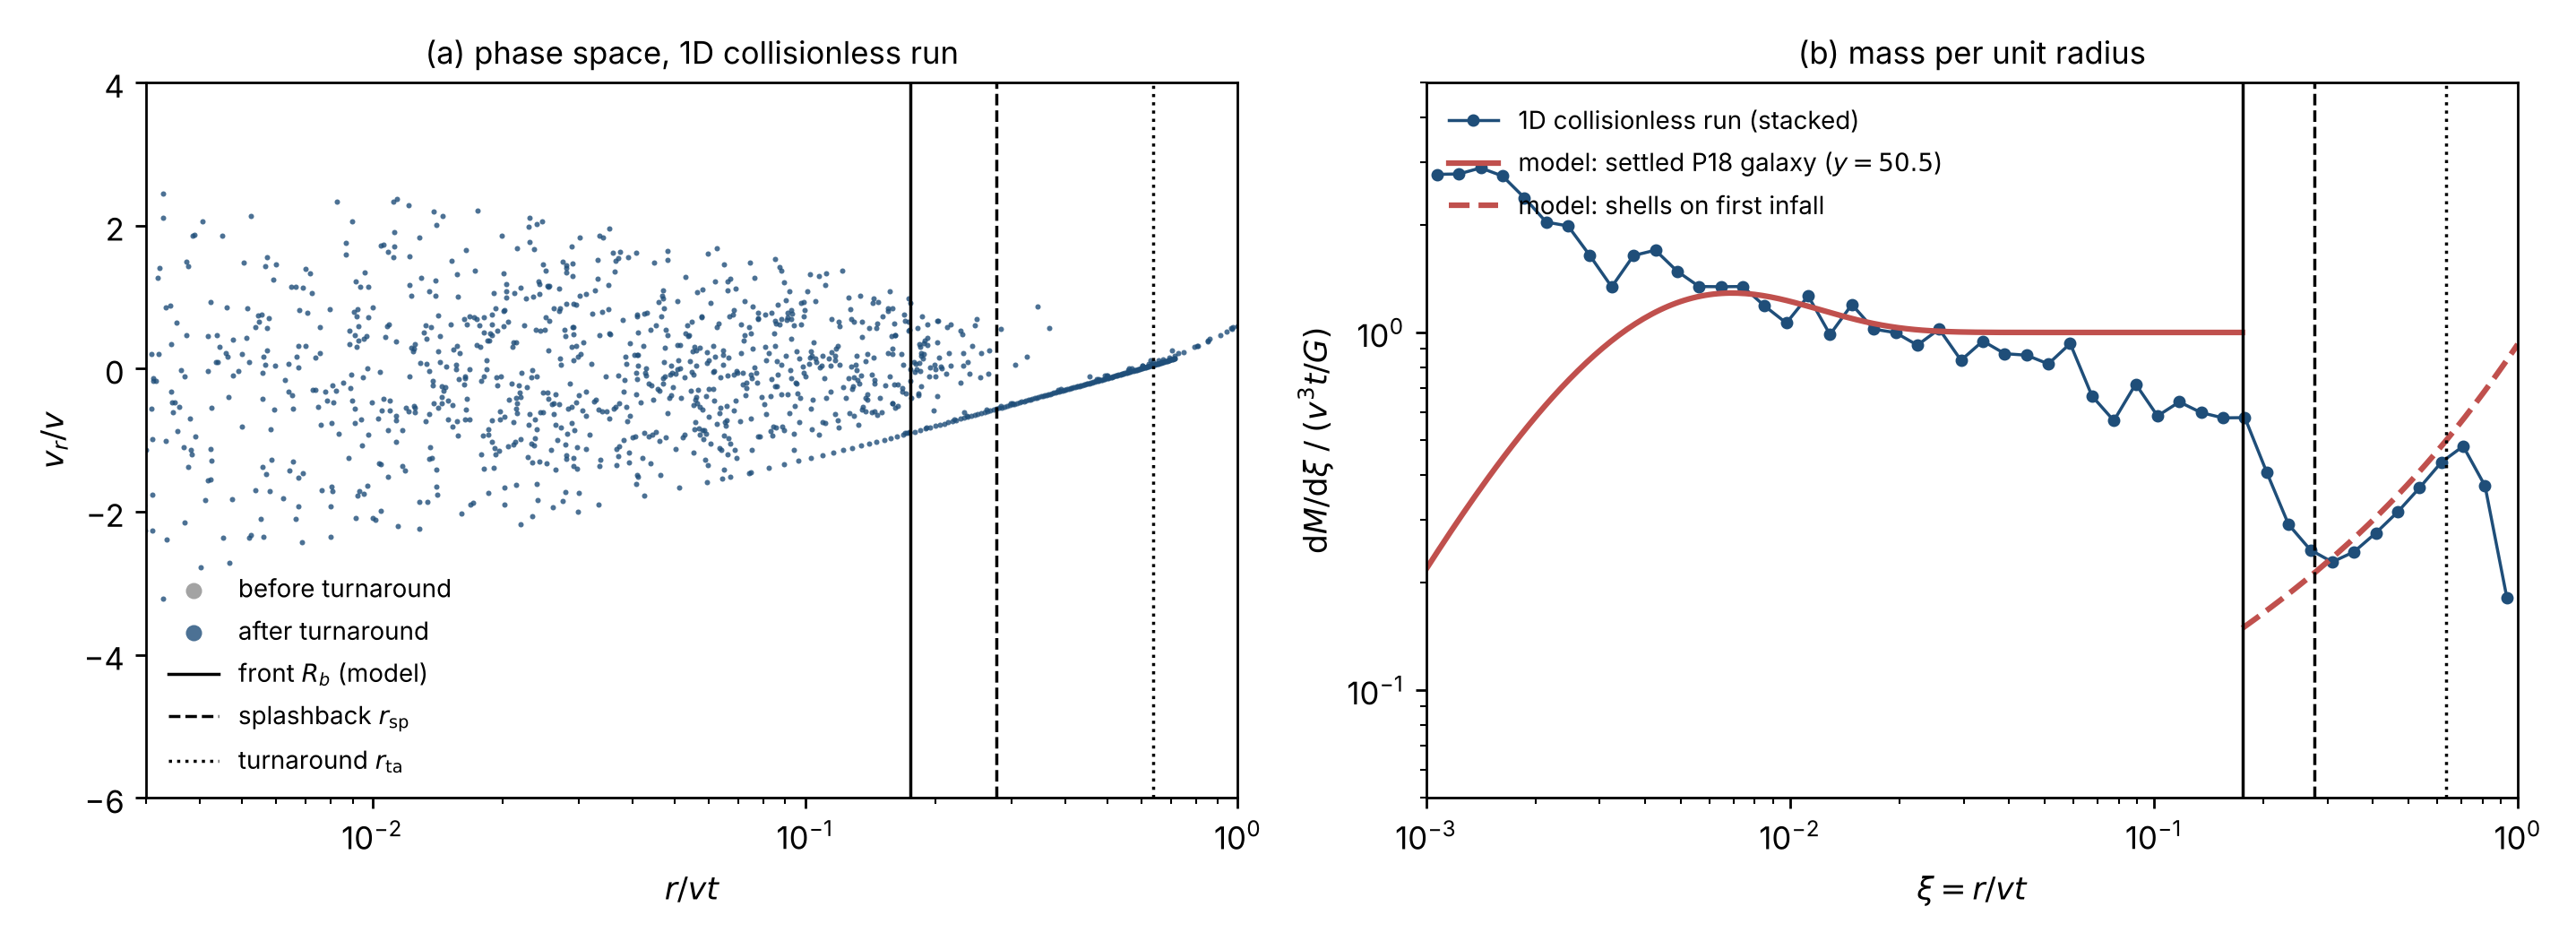
\includegraphics[width=\textwidth]{fig_splashback.png}
\caption{Our seed without halting. (a) Phase space of the last snapshot
of the one-dimensional collisionless run: radial velocity against radius;
grey, shells before turnaround; blue, after turnaround. The coherent
stream from upper right to lower left is matter on its first infall;
the cloud inside is the orbiting, multistream matter. (b) Mass per unit
$\xi=r/vt$, stacked over nine snapshots (points), against the model of
the main paper: the settled P18 galaxy inside the front (solid) and the
cycloid infall outside it (dashed). Vertical lines: the front $\Rb$ of
the model (solid), the outer edge of the orbiting matter, $\rsp$
(dashed), and the current turnaround radius (dotted).}
\label{fig:splash}
\end{figure}

\paragraph{Phase space.} Panel (a) shows the structure of every
self-similar collisionless halo: a single cold stream of infalling
matter, which turns around at $\rta$ and falls in with increasing speed,
and inside a hot cloud of orbiting matter with radial velocities up to
about $\pm2v$. The cloud ends near $\xi\simeq0.3$, beyond the front of
our model at $\xi_b=0.175$.

\paragraph{Numbers.} The analysis script gives:
\begin{itemize}
\item the steepest drop of the density outside the front at
  $\xi=0.204$, with a logarithmic slope of $-4.5$, i.e.\ at
  $1.17\,\Rb$ or $0.32\,\rta$: the splashback feature as simulations
  define it;
\item the radius enclosing 99\% of the orbiting mass at
  $\xi=0.276\pm0.009$, i.e.\ $1.58\,\Rb$ or $0.43\,\rta$: the outer edge
  of the orbits;
\item $15\pm2\%$ of the orbiting mass outside the front $\Rb$.
\end{itemize}
The first number falls inside the range expected from the calibration of
simulated haloes, $(1.1$--$1.3)\,\Rb$; both lie at about a third of the
current turnaround radius, like the outermost caustic of
\citet{Bertschinger1985}.

\paragraph{Profiles.} Panel (b) compares the run with our model. Outside
$\xi\simeq0.3$ the two agree: the infalling stream is the same cycloid
in both. Between the front and $\rsp$ the run has orbiting matter where
the model has only infall; the model's discontinuity at $\Rb$ is spread
over the splashback zone. Inside, the run follows the isothermal
$\dd M/\dd\xi\approx$ const, slightly steeper towards the centre, and has
no core; this is the failure of settling in spherical symmetry discussed
in the main paper.

\section{What this means for our model}

\paragraph{(A3) is a sticky version of splashback.} The halting condition
(A3) stops each shell on its first infall at half its turnaround radius
and keeps it there. Collisionless matter does not stop; it oscillates
out to the splashback radius. Both pictures conserve mass across the
boundary, and both put the edge of the multistream region at a fixed
fraction of the current turnaround radius, which is what makes our front
move at a constant speed. Our front is the inner edge of the splashback
zone, close to the virial radius; the true outer edge of the orbiting
matter lies at $1.2$--$1.6\,\Rb$.

\paragraph{The unrelaxed layer.} The energy budget of the main paper
(its Table~1) contains a term for the matter that has crossed the front
recently and may not yet be distributed as P18 assumes; it estimated
the fraction of such matter as $\xi_b\simeq17\%$. The run gives an
independent number: $15\%$ of the orbiting matter lies outside the front.
The two agree, which supports the size of that term, though not the
assumed 5\% error in its gravitational energy.

\paragraph{The infall profile.} Outside the splashback zone the model's
infalling density, the cycloid profile of the main paper, is not an
approximation: the collisionless run follows it.

\paragraph{Observability.} For the example galaxy of the main paper
($\Rb=84$\,kpc at the end of growth) the splashback radius would lie at
about 100--130\,kpc, far beyond any rotation curve. Only stacked weak
lensing reaches such radii; for isolated galaxies, mostly more massive
than our dwarfs, it shows circular speeds that stay flat to about
300\,kpc without an edge \citep{Mistele2024}.

\begin{thebibliography}{99}
\bibitem[Adhikari et al.(2014)]{Adhikari2014} Adhikari, S., Dalal, N., \& Chamberlain, R.~T. 2014, JCAP, 11, 019
\bibitem[Bertschinger(1985)]{Bertschinger1985} Bertschinger, E. 1985, ApJS, 58, 39
\bibitem[Diemer(2022)]{Diemer2022} Diemer, B. 2022, MNRAS, 513, 573
\bibitem[Diemer \& Kravtsov(2014)]{Diemer2014} Diemer, B., \& Kravtsov, A.~V. 2014, ApJ, 789, 1
\bibitem[Fillmore \& Goldreich(1984)]{Fillmore1984} Fillmore, J.~A., \& Goldreich, P. 1984, ApJ, 281, 1
\bibitem[Mistele et al.(2024)]{Mistele2024} Mistele, T., McGaugh, S., Lelli, F., Schombert, J., \& Li, P. 2024, ApJ, 969, L3
\bibitem[More et al.(2015)]{More2015} More, S., Diemer, B., \& Kravtsov, A.~V. 2015, ApJ, 810, 36
\end{thebibliography}

\appendix
\section{Code}
The run: \texttt{code/splashback\_run.py}, which uses the shell
integrator \texttt{code/shells.py} of the main paper (about four
minutes); the analysis and figure: \texttt{code/splashback\_fig.py}.
\lstinputlisting{code/splashback_run.py}
\lstinputlisting{code/splashback_fig.py}
Output of the analysis:
\lstinputlisting[language={}]{code/splashback_fig_output.txt}
\end{document}
